% chap2.tex
\chapter{掌面積・体積評価手法}

\section{掌面積・体積評価の必要性}

本研究では、災害時における河川水等を介した病原微生物への曝露を想定し、
掌に付着するウイルス量および洗浄後の残存量を定量的に評価することを目的としている。
手指を介した感染リスクを評価するためには、単に回収された微生物量を比較するだけでなく、
被験者間の掌の大きさの違いを考慮した上で、
付着量や残存量を適切に比較・解析する必要がある。

掌の面積や体積は個人差が大きく、同一条件下で実験を行った場合であっても、
掌の大きさの違いにより付着水量や微生物の付着量が異なる可能性がある。
そのため、掌面積あるいは体積を指標として用い、
得られたデータを標準化することは、
被験者間の比較を行う上で不可欠である。

特に、本研究では後述するウイルス付着実験および洗浄実験において、
掌に付着した水分量およびウイルス量を定量的に評価し、
さらに統計解析やリスク評価へと展開する。
この際、掌面積および体積の情報は、
水分付着量の正規化やウイルス残存率の算定における
基礎データとして重要な役割を果たす。

以上の理由から、本章では後続章で実施する各種実験および解析の前提条件として、
掌面積および体積を算出するための測定条件および解析手法について詳細に検討する。
一律な実験条件下において被験者の掌への付着量を正確に測定・分析するための基盤として、
本章で示す手法を確立することを目的とする。

%--------------------------------------------------

\section{実験材料}

本研究における掌面積および体積の測定には、以下の器具を使用した。

\begin{itemize}
  \item ノギス  
  掌の厚みを測定するために使用した。
  \item フラットベッドスキャナー（Canon CanoScan）  
  掌の形状を平面画像として取得するために使用した。
  \item 定規（10 cm 以上）  
  スキャン画像における実寸スケールを設定するために使用した。
  \item 画像処理ソフト（ImageJ）  
  スキャン画像から掌面積を算出するために使用した。
\end{itemize}

これらの器具を組み合わせることで、
掌の平面形状および厚み情報を取得し、
面積および体積の定量化を行った。

%--------------------------------------------------

\section{実験方法および測定条件}

被験者は学生8名および教員1名の計9名とし、
すべて同一条件下で測定を行った。
掌面積の測定は、各被験者について左右の手それぞれ3回ずつ
スキャナーで測定し、
1人あたり計6セットのデータを取得した。

\subsection{掌画像の取得}

掌をスキャナーのガラス面に軽くのせ、
掌全体が写るように自然に広げた状態でスキャンを行った。
この際、実寸スケールの基準とするため、
定規を掌の横に配置して同時にスキャンした。

\subsection{画像データの保存}

取得したスキャン画像はパーソナルコンピュータに保存した。
画像の解像度は300～600\,dpi 程度とし、
掌の輪郭が明瞭に判別できる条件とした。

\subsection{ImageJによるスケール設定}

ImageJを用いてスキャン画像を開き、
定規上の既知長（5\,cm）を直線ツールで指定した後、
スケール設定を行った。
これにより、画像上のピクセル数を
実寸（cm）に変換可能とした。

\subsection{掌面積の算出}

掌の外周をポリゴン選択または
フリーハンド選択ツールで囲み、
ImageJの測定機能を用いて
掌面積（cm$^2$）を算出した。

\subsection{補助測定および注意点}

ノギスを用いて手長および手幅を測定し、
算出した面積値との整合性を確認した。
測定精度を高めるため、
複数回のスキャン結果を平均値として評価した。
また、掌の湿り気や体温による
ガラス面の曇りが誤差要因となるため、
各測定ごとにガラス面を清拭した。

%--------------------------------------------------

\section{掌体積推定を行う理由}

掌体積の推定を行う理由は、
ウイルス付着量を掌表面のみならず、
立体的な形状を考慮した指標として評価するためである。
特に、掌の厚みによって水分保持量が変化する可能性を考慮すると、
掌を平面形状のみで評価することは十分ではない。

そのため、本研究では掌を立体構造として捉え、
体積情報を取得することで、
付着水量やウイルス付着量を
より多面的に議論することを目的とした。

%--------------------------------------------------

\section{掌体積の算出方法}

掌の体積は、形状やしわの個人差が大きく、
厳密に表現することが困難である。
そこで本研究では、掌を複数の領域に分割し、
「領域ごとの面積と厚み」を用いた近似法により
体積を推定した。

具体的には、掌をA～Gの7領域に区分し、
各領域内の代表的な20か所について
ノギスを用いて掌厚を測定した。
測定箇所の概略を図\ref{fig:hand_thickness_points}に示す。
これらの測定値から領域ごとの平均厚みを算出し、
同領域のスキャナー画像から求めた面積と乗じることで、
領域体積を求めた。

体積推定式を以下に示す。

\begin{equation}
V_i = A_i \times T_i
\end{equation}

ここで、$A_i$ は領域 $i$ の面積（cm$^2$）、
$T_i$ は同領域の平均厚み（cm）である。

参考例として、被験者Aにおける掌厚測定結果および
領域体積算出結果を表\ref{tab:hand_region_thickness}に示す。

\begin{figure}[htbp]
  \centering
  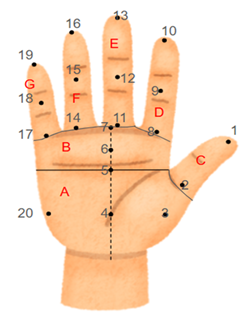
\includegraphics[width=0.4\textwidth]{fig/hand_thickness_points.png}
  \caption{掌測定箇所}
  \label{fig:hand_thickness_points}
\end{figure}

\begin{table}[htbp]
  \centering
  \caption{被験者Aにおける掌領域別厚み測定結果および体積算出例}
  \label{tab:hand_region_thickness}
  \begin{tabular}{c c c c c}
    \hline
    測定箇所 & 厚み (mm) & 平均厚み (mm) & 面積 (cm$^2$) & 体積 (cm$^3$) \\
    \hline
    1  & 16.9  &        &        &        \\
    2  & 18.35 & 17.63  & 15.873 & 27.976 \\
    \hline
    3  & 41.0  &        &        &        \\
    4  & 46.9  &        &        &        \\
    20 & 40.5  & 42.80  & 61.918 & 265.008 \\
    \hline
    5  & 35.025 &        &        &        \\
    6  & 29.8   &        &        &        \\
    7  & 25.07  & 29.97  & 37.673 & 112.886 \\
    \hline
    8  & 19.1  &        &        &        \\
    9  & 14.8  &        &        &        \\
    10 & 13.5  & 15.80  & 14.823 & 23.421 \\
    \hline
    11 & 19.1  &        &        &        \\
    12 & 14.8  &        &        &        \\
    13 & 13.5  & 15.80  & 17.131 & 27.066 \\
    \hline
    14 & 17.0  &        &        &        \\
    15 & 13.5  &        &        &        \\
    16 & 12.0  & 14.17  & 14.451 & 20.472 \\
    \hline
    17 & 14.7  &        &        &        \\
    18 & 12.25 &        &        &        \\
    19 & 10.9  & 12.62  & 11.994 & 15.132 \\
    \hline
    \multicolumn{4}{r}{総体積 (cm$^3$)} & 491.962 \\
    \hline
  \end{tabular}
\end{table}

%--------------------------------------------------

\section{測定結果}

掌面積の測定は、左右それぞれ3回ずつ実施し、
その平均値を各被験者の代表値とした。
複数回測定を行った理由は、
スキャナーの読み取り誤差や
手の置き方によるばらつきを低減し、
再現性および信頼性の高いデータを得るためである。

各被験者の左右の平均掌面積および掌体積を
表\ref{tab:hand_area_volume}に示す。

\begin{table}[htbp]
  \centering
  \caption{被験者ごとの掌面積および掌体積}
  \label{tab:hand_area_volume}
  \begin{tabular}{c|cc|cc}
    \hline
    被験者名 & \multicolumn{2}{c|}{掌の面積 (cm$^2$)} & \multicolumn{2}{c}{掌の体積 (cm$^3$)} \\
             & 右 & 左 & 右 & 左 \\
    \hline
    A & 172.88  & 167.13  & 491.96  & 479.67 \\
    B & 136.88  & 136.75  & 358.86  & 349.48 \\
    C & 134.15  & 138.25  & 338.22  & 335.20 \\
    D & 143.46  & 137.52  & 352.03  & 316.30 \\
    E & 136.88  & 134.00  & 357.28  & 326.40 \\
    F & 153.90  & 148.56  & 306.57  & 311.32 \\
    G & 136.99  & 139.09  & 342.12  & 349.95 \\
    H & 137.88  & 137.81  & 406.86  & 336.94 \\
    I & 135.17  & 129.81  & 256.38  & 223.61 \\
    \hline
  \end{tabular}
\end{table}

%--------------------------------------------------

\section{掌面積および体積の左右差に関する解析結果}

9名の被験者を対象として、
左右の掌面積および体積の差について解析を行った。
解析には対応のある$t$検定を用い、
有意水準は5\%（$p<0.05$）とした。

その結果を表\ref{tab:hand_lr_ttest}に示す。
掌面積では右手が平均でわずかに大きい傾向
（+1.5\%）を示したものの、
統計的に有意な差は認められなかった
（$p=0.127$）。
一方、掌体積では右手が平均で約6.2\%大きく、
統計的に有意な差が認められた
（$p=0.0399$）。

\begin{table}[htbp]
  \centering
  \caption{掌面積および掌体積における左右差の統計解析結果}
  \label{tab:hand_lr_ttest}
  \begin{tabular}{l c c c c c}
    \hline
    項目 & 平均差 & 左右差割合 (\%) & $t$値 & $p$値 & 有意差 \\
    \hline
    掌の面積 & 2.04\,cm$^2$ & 1.50 & 1.70 & 0.127 & なし \\
    掌の体積 & 19.93\,cm$^3$ & 6.20 & 2.45 & 0.0399 & あり \\
    \hline
  \end{tabular}
\end{table}

これらの結果から、
掌面積には有意な左右差は認められなかったが、
掌体積においては利き手側の使用頻度や
筋肉量の発達が反映されている可能性が示唆された。

%--------------------------------------------------

\section{掌面積および体積の左右差に関する考察}

本研究において、掌面積および掌体積の左右差について検討した結果、
掌面積では個人差が大きく、
利き手による影響は統計的に明確ではなかった。
一方で、掌体積においては
右手が有意に大きい結果が得られた。

掌体積に有意な左右差が認められた要因として、
利き手側の使用頻度の高さや
筋肉量の発達が掌の厚みに反映された可能性が考えられる。
日常生活において利き手は非利き手に比べて使用頻度が高く、
把持動作や荷重が繰り返されることから、
筋組織や軟部組織の発達が
掌体積の増加として現れた可能性が高い。

一方、掌面積については
有意な左右差が認められなかった。
掌面積は骨格構造や手の外形に依存する形態的指標であり、
日常的な使用による変化が生じにくいと考えられる。
そのため、利き手・非利き手間においても
統計的に有意な差が
現れなかったものと推察される。

これらの結果は、
利き手優位性（hand dominance）に関する
既存の知見とも整合的であり、
機能的な使用頻度の違いが
厚みや体積といった立体的指標に反映されやすい一方で、
平面的な形状には
反映されにくいことを示唆している。

本研究では被験者数が限られているため、
利き手の影響を十分に一般化するには至らない。
今後は被験者数を増加させるとともに、
利き手情報を明確に取得したうえで解析を行うことで、
利き手と非利き手の
構造的および機能的差異を
より詳細に評価できると考えられる。

%--------------------------------------------------

\section{本章のまとめ}

本章では、後続章におけるウイルス付着実験および洗浄実験に先立ち、
掌面積および体積を定量的に評価する手法を確立した。
これにより、被験者間の身体的差異を考慮した
付着量および残存量の比較が可能となり、
以降の解析およびリスク評価の基盤が整えられた。
